\section{Perancangan Antar Muka Aplikasi}
Aplikasi \emph{question answering} yang akan dikembangkan dalam penelitian ini hanya memiliki satu buah halaman antar seperti terlihat pada gambar \ref{fig:rancangan_antarmuka}. Masukan pertanyaan dan jawaban diletakkan dalam satu buah halaman yang sama. Pada tahap awal sebelum pengguna mengirimkan pertanyaan hanya akan disediakan sebuah \emph{field} dengan tipe \emph{text} dan sebuah tombol submit yang berfungsi untuk mengirimkan pertanyaan ke sever.

\begin{figure}[hb]
    \centering
    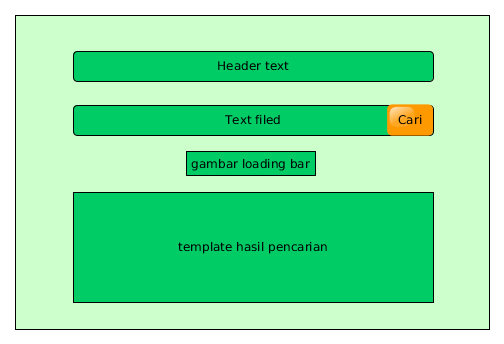
\includegraphics[width=1\textwidth]{rancangan_antar_muka}
    \caption{Rancangan antar muka aplikasi \emph{question answering} data kabupaten di Nusa Tenggara Barat}
    \label{fig:rancangan_antarmuka}
\end{figure}

Bagian header berisi nama dari aplikasi \emph{question answering}, kemudian dibawahnya terdapat sebuah text field yang digunakan untuk memasukkan pertanyaan. Atribut \emph{placeholder} dari input field diisi dengan tulisan ``Masukkan pertanyaan'' untuk memudahkan pengguna memahami bagian input field itu sendiri. Selanjutnya, di sebelah input filed terdapat sebuah tombol yang digunakan untuk melakukan submit form.

Bagian bawah input form diletakkan sebuah gambar ``loading bar'' yang berfungsi untuk memberitahuan kepada user bahwa proses pencarian jawaban sedang berlangsung. Gambar ini akan muncul ketika pengguna telah melakukan submit form dengan cara menekan tombol ``cari'' atau dengan menekan tombol ``enter'' pada keyboard. Setelah jawaban diperoleh, maka gambar tersebut akan secara otomatis hilang dan jawaban hasil pencarian akan ditampilkan dibawahnya. Setelah jawaban ditampilkan, input filed tidak akan dikosongkan, hal ini dimaksudkan agar pengguna dapat melihat relasi antara pertanyaan yang dimasukkan dengan hasil jawaban yang didapatkan.

Pengguna dapat melakukan pencarian baru dengan cara menghapus pertanyaan sebelumnya yang terdapat pada input field untuk kemudian menggantinya dengan pertanyaan yang baru. Sesaat setelah user menekan tombol ``enter'' atau tombol ``cari'' maka bagian template hasil pencarian akan dikosongkan dan gambar ``loading bar'' akan kembali muncul seperti pada proses sebelumnya.